
本节主要介绍利用 Material Studio 2020\footnote{Material Studio 8在 Windows 11 上不能正常运行。} 对硅晶体的各项属性进行模拟计算的操作步骤与结果。

\subsection{硅晶体的构建}

硅晶体是常见的本征半导体之一,也是进行掺杂来构造其他半导体的典型基体。
其晶胞为金刚石型面心立方结构,皮尔逊表示为 cF8,室温下的晶胞参数为$a = \qty{543.0986}{\pico\metre}$。
该晶胞对应的空间群为$\mathrm{Fd\overline{3}M}$,表示面心布拉伐格点(F)、金刚石型平移对称(d)、旋转反演角为$\frac{\ang{360}}{3}=\ang{120}$、镜像面与转轴垂直(M)。
图~\ref{fig:silicon-cell}~展示了硅晶体的晶胞与原胞,其中晶格参数即为红色立方体的边长。

\begin{figure}[ht!]
    \centering
    \begin{asy}
        \input{silicon-cell.asy}
    \end{asy}
    \caption{硅晶体的晶胞(红色)与原胞(蓝色)}\label{fig:silicon-cell}
\end{figure}

为在 Material Studio 中为该分子建模,首先新建原子结构文件(3D Atomistic),然后在下拉菜单中选择构造(Build)、晶体(Crystal)、构造晶体(Build crystal)。
在新对话框中输入晶体的空间群,然后输入晶格参数,即可完成晶胞的构建。
然后,向其中加入原子,选择构造(Build)、添加原子(Add Atoms)并填入原子的元素符号,即可在晶胞中填充原子。
图~\ref{fig:ms-cells}~展示了 Material Studio 中构建的晶体。

\begin{figure}
    \centering
    \begin{subfigure}[c]{0.4\linewidth}
        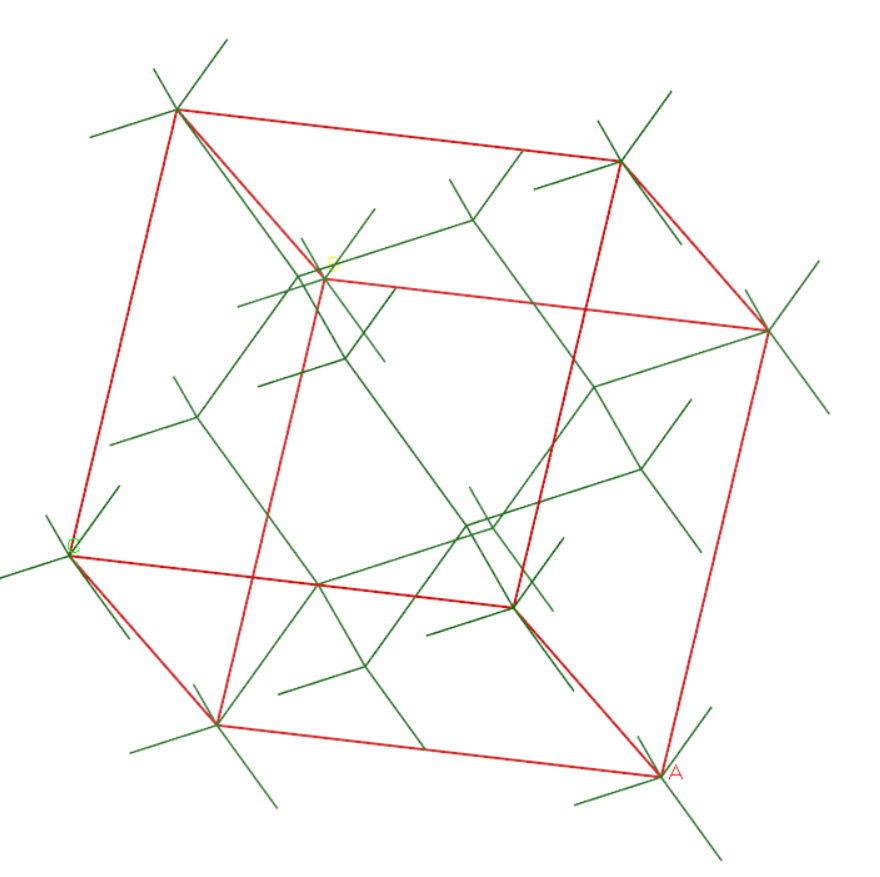
\includegraphics[width=\linewidth]{screenshots/unit-cell.png}
    \end{subfigure}
    \begin{subfigure}[c]{0.4\linewidth}
        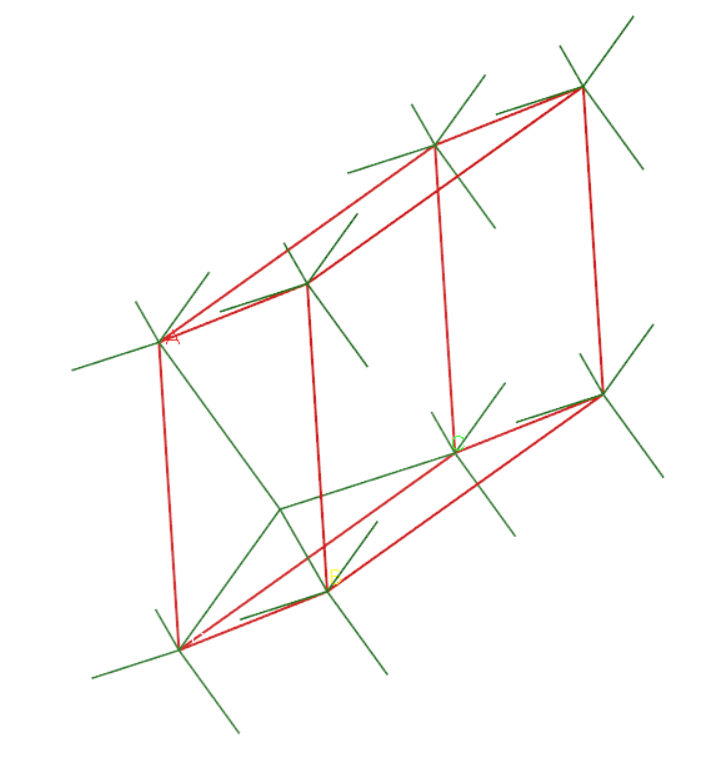
\includegraphics[width=\linewidth]{screenshots/primitve-cell.png}
    \end{subfigure}
    \caption{Material Studio 中的晶体}\label{fig:ms-cells}
\end{figure}

\subsection{布里渊区与 K 路径}

我们考虑金刚石型晶体——或更一般的,面心立方晶体的布里渊区的结构。

\begin{proposition}
    面心立方晶体的(第一)布里渊区是倒空间中的截角八面体(truncated octahedron),即从正八面体的角上截去六个相同的四棱锥形成的多面体,如图~\ref{fig:truncated-octahedron}所示。
\end{proposition}

\begin{figure}[ht!]
    \centering
    \input{truncated-octahedron.asy}
    \caption{倒空间中的截角八面体}
    \label{fig:truncated-octahedron}
\end{figure}

\begin{proof}
    不妨设面心立方晶胞的边长为$\frac{2}{\pi}$,考虑正空间中的原胞产生的格点的基底
    \begin{equation}
        a_1 = (\frac{1}{\pi}, \frac{1}{\pi}, 0), \; a_2 = (\frac{1}{\pi}, 0, \frac{1}{\pi}), \; a_3 = (0, \frac{1}{\pi}, \frac{1}{\pi}).
    \end{equation}
    对应的倒空间基底自然为
    \begin{equation}
        b_1 =  (1, 1, -1), b_2 = (1, -1, 1), b_3 = (- 1, 1, 1).
    \end{equation}
    由于原胞的基底不正交,倒空间的基底也不正交,其立体夹角为
    \begin{equation}
        \phi = \arccos \frac{b_1 \cdot b_2}{\Vert b_1 \Vert \cdot \Vert b_2 \Vert} \approx \ang{109.47}.
    \end{equation}
    我们现在仅考虑一个卦限中的情况,其他情况可容易地根据对称性推出,考虑与原点紧邻的七个格点,首先在倒空间基底中写出其坐标:
    \begin{equation}
        \begin{aligned}
            A(1, 0, 0), B(0, 1, 0), C(0, 0, 1), D(1, 1, 1) \\
            E(1, 1, 0), F(1, 0, 1), G(0, 1, 1), 
        \end{aligned}
    \end{equation}
    然后回到笛卡尔坐标系中,首先注意$A, B, C, D$:
    \begin{equation}
        A' (1, 1, -1), B' (1, -1, 1), C'(-1, 1, 1), D'(1, 1, 1),
    \end{equation}
    从原点到这四个点的连线的垂直平分面截成了正八面体的一部分,而剩下三个点的垂直平分面则从这个正八面体中截除了全等的三个四棱锥。
\end{proof}

\subsection{计算能带}
